\documentclass[11 pt]{article}

\usepackage{amsmath}
\usepackage[left=2cm,right=2cm,top=2cm,bottom=2cm]{geometry}
\usepackage{fancyhdr}
\usepackage{graphicx}
\usepackage{listings}
\usepackage{xcolor}

\pagestyle{fancy}
\fancyhf{}
\lhead{Fundamentals of Simulation Methods}
\chead{Exercise 02}
\rhead{V. Mader}
\setlength{\headheight}{15pt}

\definecolor{commentsColor}{rgb}{0.497495, 0.497587, 0.497464}
\definecolor{keywordsColor}{rgb}{0.000000, 0.000000, 0.635294}
\definecolor{stringColor}{rgb}{0.558215, 0.000000, 0.135316}
\lstset{ %
  backgroundcolor=\color{white},   % choose the background color; you must add \usepackage{color} or \usepackage{xcolor}
  basicstyle=\footnotesize,        % the size of the fonts that are used for the code
  breakatwhitespace=false,         % sets if automatic breaks should only happen at whitespace
  breaklines=true,                 % sets automatic line breaking
  captionpos=b,                    % sets the caption-position to bottom
  commentstyle=\color{commentsColor}\textit,    % comment style
  deletekeywords={...},            % if you want to delete keywords from the given language
  escapeinside={\%*}{*)},          % if you want to add LaTeX within your code
  extendedchars=true,              % lets you use non-ASCII characters; for 8-bits encodings only, does not work with UTF-8
  frame=tb,	                   	   % adds a frame around the code
  keepspaces=true,                 % keeps spaces in text, useful for keeping indentation of code (possibly needs columns=flexible)
  keywordstyle=\color{keywordsColor}\bfseries,       % keyword style
  language=Python,                 % the language of the code (can be overrided per snippet)
  otherkeywords={*,...},           % if you want to add more keywords to the set
  numbers=left,                    % where to put the line-numbers; possible values are (none, left, right)
  numbersep=5pt,                   % how far the line-numbers are from the code
  numberstyle=\tiny\color{commentsColor}, % the style that is used for the line-numbers
  rulecolor=\color{black},         % if not set, the frame-color may be changed on line-breaks within not-black text (e.g. comments (green here))
  showspaces=false,                % show spaces everywhere adding particular underscores; it overrides 'showstringspaces'
  showstringspaces=false,          % underline spaces within strings only
  showtabs=false,                  % show tabs within strings adding particular underscores
  stepnumber=1,                    % the step between two line-numbers. If it's 1, each line will be numbered
  stringstyle=\color{stringColor}, % string literal style
  tabsize=2,	                   % sets default tabsize to 2 spaces
  title=\lstname,                  % show the filename of files included with \lstinputlisting; also try caption instead of title
  columns=fixed                    % Using fixed column width (for e.g. nice alignment)
}


\begin{document}

    \section{Pitfalls of pseudo-random number generation}
        Consider the linear congruential random number generator RANDU,
        introduced by IBM in System/3660 mainframes i nthe early 60s. 
        (Donald Knuth called this random number generator "really horrible",
        and it is indeed notorious for being one of the worst generators
        of all time). The recursion relation of RANDU is defined by 
        \begin{equation}
            I_{i+1}=(65539\cdot I_i)\textnormal{ mod }2^{31}
        \end{equation}
        and needs to be started from an odd integer. The obtained integer 
        values can be mapped to pseudo-random floating point numbers 
        $u_i\in[0,1]$ through
        \begin{equation}
            u_i=I_i / 2^{31}
        \end{equation}

        \paragraph{a) Implement this number generator. Make sure that you do 
            not use the 32-bit integer arithmetic, otherwise overflows will 
            occur.  (Use 64-bit integer arithmetic instead, or double precision 
            for simplicity - its precision is sufficient to represent the 
            relevant integer range exactly)
        } \ \\
        \\
        The next "random" integer can be generated from a given input integer 
        via the following python code:
        \begin{lstlisting}
            from numpy import uint64, power
            
            def get_next_RANDU_int(previous_int):
                # make sure all variables are 64-bit floats
                previous_int = uint64(previous_int)
                a = uint64(65539)
                b = uint64(2)
                c = uint64(31)
            
                return (a * previous_int) % power(b, c)\end{lstlisting}

        \paragraph{b) Now generate 2-tuples of successive random numbers from 
            the sequence generated by the generator, i.e. 
            $(x_i,y_i)=(u_{2i},u_{2i+1})$. Generate 1000 points and make a 
            scatter plot of the points in the unit square. Does this look 
            unusual? How does this look in 3D (using 3-tuples)?
        } \ \\
        \\
        First, we create a list of the first 1000 "random" integers. The 
        first entry in this list is 1, the remaining entries can be calculating
        using the function we just defined above.
        \begin{lstlisting}
            def get_list_of_N_random_ints(N):
                list_of_random_ints = [uint64(1)]
            
                for _ in range(N):
                    i = list_of_random_ints[-1]
                    j = get_next_RANDU_int(i)
                    list_of_random_ints.append(j)
            
                return list_of_random_ints

            first_1000_ints = get_list_of_N_random_ints(1000)\end{lstlisting}
        \newpage \noindent
        Now we can convert the integers to floating point numbers and 
        create a list of tuples. For this, we need a "normalization" function 
        which takes an integer and converts it to a float between 0 and 1 
        (by dividing it by $2^{31}$): \ \\
        \begin{lstlisting}
            def normalize(num):
                return num / power(uint64(2), uint64(31))
            
            def get_list_of_N_float_tuples(N):
                list_of_random_float_tuples = []
                list_of_random_ints = get_list_of_N_random_ints(N+1)
            
                for idx, item in enumerate(list_of_random_ints[:-1]):
                    a, b = item, list_of_random_ints[idx + 1]
            
                    list_of_random_float_tuples.append(
                        (normalize(a), normalize(b))
                    )
            
                return list_of_random_float_tuples\end{lstlisting} \ \\
        \\
        Let us now plot these points.
        \begin{lstlisting}
            import matplotlib.pyplot as plt

            def plot_points():
                list_of_random_float_tuples = get_list_of_N_float_tuples(1000)

                x = [i[0] for i in list_of_random_float_tuples]
                y = [i[1] for i in list_of_random_float_tuples]

                plt.figure(figsize=(4, 4))
                plt.xlim(0, 1)
                plt.ylim(0, 1)
                plt.xlabel('x')
                plt.ylabel('y')
                plt.scatter(x, y, color='red', s=3)
                plt.savefig('fig1.pdf')
                plt.close()\end{lstlisting} \ 
        \\
        The resulting figure can be seen on the next page.
        \newpage
        \begin{figure}[h!]
            \centering
            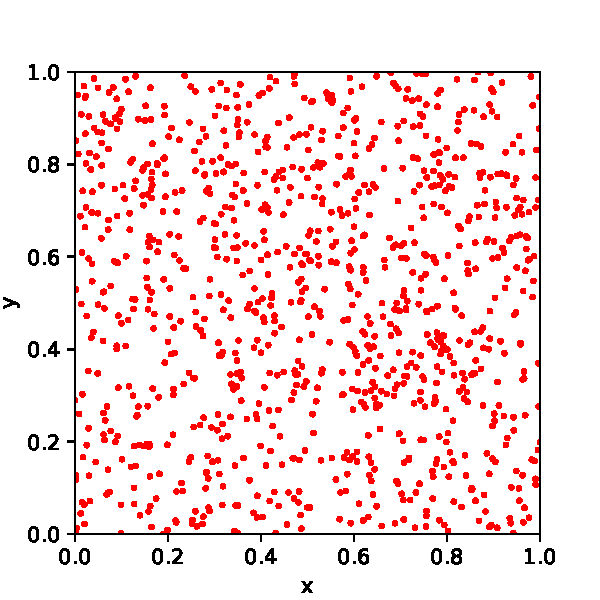
\includegraphics[width=0.5\textwidth]{./code/fig1.pdf} 
            \caption{Plot for task 1b)}
        \end{figure}


        \paragraph{c) Now zoom in by a large factor onto a small region of the 
            square, for example $[0.2,0.201]\times[0.3,0.301]$ and generate 
            enough points that there are again 1000 points within the small 
            region as before. Interpret the results.
        } \ \\
        \\ 

        \paragraph{d) Repeat a) - c) for you favorite standard RNG.}

    \newpage
    \section{Performance of Monte Carlo integration in different dimensions}
        We would like to compare the performance of the Monte Carlo integration
        technique with the regular midpoint method. To this end, consider the 
        integral
        \begin{equation}
            I=\int_Vf(\vec x)\cdot\textnormal{d}^d\vec x
        \end{equation}
        where the integration domain $V$ is a $d$-dimensional hypercube with 
        $0\leq x_i\leq1$ for each component of the vector 
        $\vec x=(x_1,x_2,..., x_d)$. The function we want to integrate is 
        given by 
        \begin{equation}
            f(\vec x)=\prod_{i=1}^d\frac{3}{2}\cdot\bigg(1-x_i^2\bigg)
        \end{equation}
        This has an analytic solution of course, which is $I=1$ independent of 
        $d$, but we want to ignore this for the moment and use the problem 
        as a test of the relative performance of Monte Carlo integration and 
        ordinary integration techniques. To this end, calculate the integral
        in dimensions $d=1,2,3,...,10$ using 

        % n = 6
        % N = 20000
        % d = 1,2,...,10     -> plot computation time as function of d

        \paragraph{a) ...the midpoint method, where you divide the volume 
            into a set of much smaller hypercubes obtained by subdividing each 
            axis into $n$ intervals, and where you approximate the integral by 
            evaluating the function at the centers of the small cubes.
        } \ \\
        \\ 

        \paragraph{b) ...standard Monte Carlo integration in $d$ dimensions, 
            using $N$ random vectors (don't use the "wrong" RNG from the 
            previous problem!)
        } \ \\

    \newpage
    \section{Probability transformation \& Metropolis Monte Carlo}
        In this exercise you are asked to transform a flat probability
        distribution
        \begin{equation}
            p(x)=\begin{cases}
                1&\textnormal{ if }x\in[0,1] \\
                0&\textnormal{ otherwise}
            \end{cases}
            \label{}
        \end{equation}
        into a distribution of the form $p_\textnormal{new}=1/x^2$, realized 
        on the interval $[1,20]$.

        \paragraph{a) Derive an \textit{exact inversion}, so that $y(x)$ is 
            distributed according to $p_\textnormal{new}(x)$ if $x$ is drawn 
            from the flat distribution.
        } \ \\
        \\

        \paragraph{b) Use the Metropolis Monte Carlo formalism to achieve the
            same goal numerically, that is: Create a set of one million random 
            numbers, distributed according to $p_\textnormal{new}(x)$ by 
            starting at an arbitrary point in $[1,20]$ and accepting/dumping new
            points based on the acceptance criterion you learned about in the 
            script/lecture. To generate new points we suggest using a normal 
            distribution: $x_{i+1}=N(x_i,\sigma)$ with step size $\sigma=0.1$,
            but you can also choose other options.
        } \ \\
        \\

        \paragraph{c) Plot your results from a) and b) in the form of 
            histograms and compare to the target distribution 
            $p_\textnormal{new}(x)$. Can you observe pathological aberrations,
            if you set the step size too small for the Metropolis Monte Carlo 
            scheme?
        }

\end{document}
